\textcite{battiti_new_2017} did not report the values for the parameters $\alpha$ and $\beta$ in their paper. We performed grid search to deterimine good values for $\alpha$ and $\beta$. The data set we used was TSPLIB (\cite{reineltTSPLIBTravelingSalesman1991a}), originally a travelling salesman data set that has been used for $k$-center, which has known optimal $k$-center costs for some instances (\cite{pullan_memetic_2008}). For each parameter pair, we perform 5 trails with 5 iterations, therefore the local search is performed 25 times. We then calculate the mean percentage above the optimal cost, and plot it in a heatmap in \cref{fig:grid_search_heatmap}.

\begin{figure}[H]
    \centering
    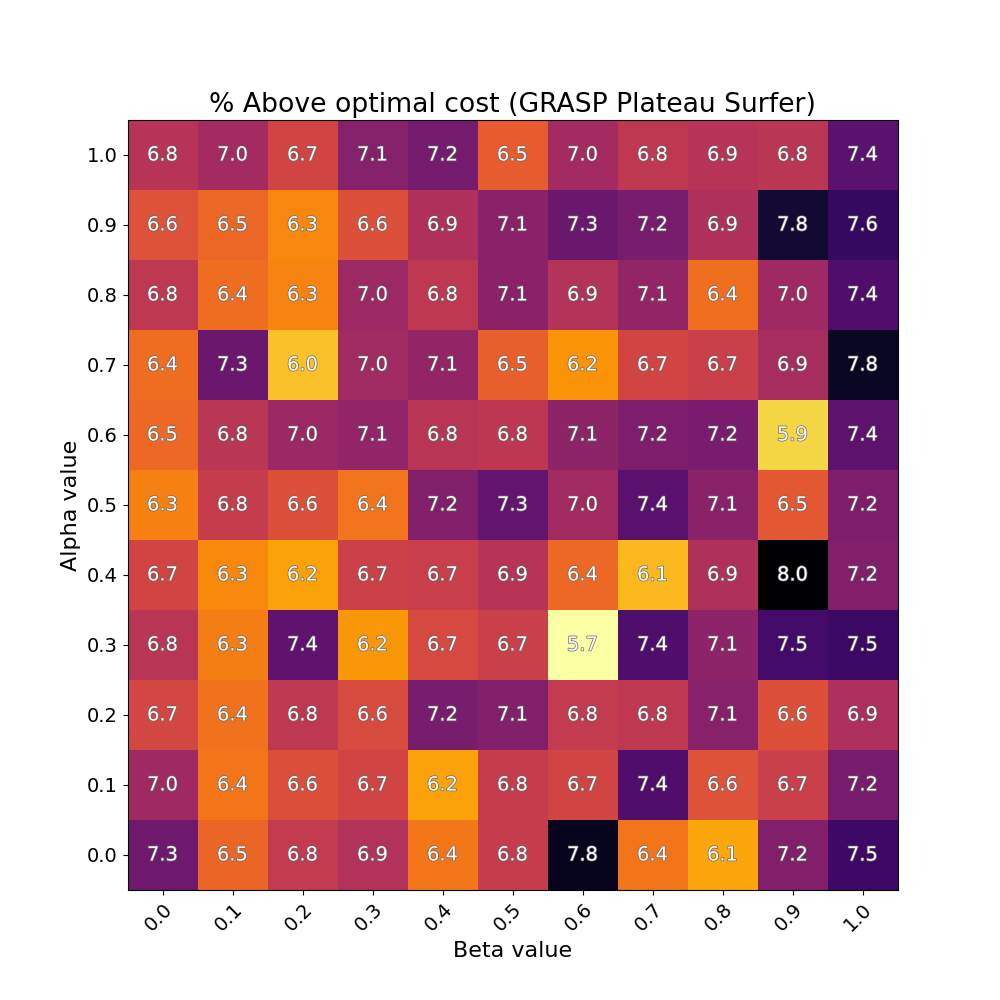
\includegraphics[height=13cm]{images/grasp_heatmap.png}
    \caption{Grasp Plateau Surfer grid search}
    \label{fig:grid_search_heatmap}
\end{figure}

The average percentage above optimal cost for each quadrant is shown in \cref{fig:grid_search_quadrant}. From this graph we concluded that an $\alpha$ and $\beta$ between $0.0-0.5$ were suitable.

\begin{figure}[H]
    \centering
    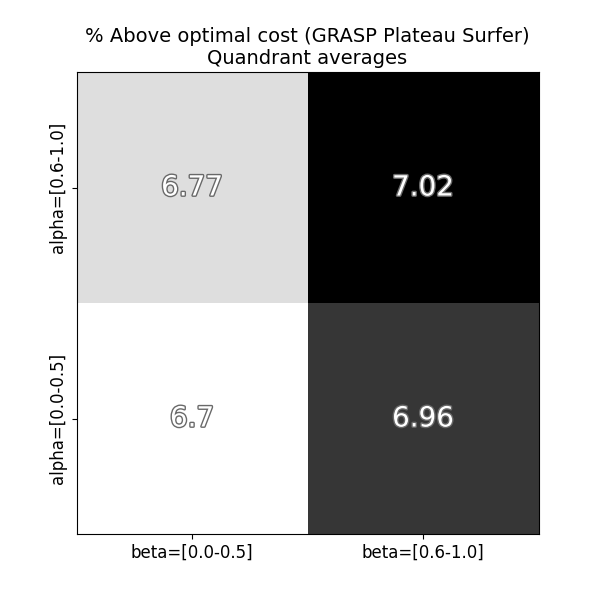
\includegraphics[height=6.5cm]{images/quadrant_averages_grasp.png}
    \caption{Grasp Plateau Surfer grid search (quadrant averages)}
    \label{fig:grid_search_quadrant}
\end{figure}